\documentclass[12pt,a4paper]{report}
\usepackage[italian]{babel}
\usepackage[utf8]{inputenc}
\usepackage{parskip}        % fa in modo che ogni paragrafo sia spaziato e non abbia l'indentazione
\usepackage{hyperref}       % Per gestire i collegamenti ipertestuali
\usepackage{listings} % Pacchetto per il codice
\usepackage{xcolor} % Opzionale, per colorare il codice
\lstset{
  language=C++,             % Linguaggio
  basicstyle=\ttfamily,      % Stile del testo
  keywordstyle=\color{blue}, % Colore delle parole chiave
  commentstyle=\color{gray}, % Colore dei commenti
  stringstyle=\color{red},   % Colore delle stringhe
  numbers=left,              % Numeri di riga a sinistra
  numberstyle=\tiny,         % Stile dei numeri di riga
  stepnumber=1,              % Mostra un numero di riga per ogni riga
  breaklines=true,           % Spezza automaticamente le righe lunghe
  frame=single,              % Cornice attorno al codice
  tabsize=4                  % Imposta la dimensione del tab
}

\usepackage{amsmath,amssymb,amsthm}
\usepackage{fancyhdr}
\usepackage{indentfirst}
\usepackage{microtype}
\usepackage{mathrsfs}
\usepackage{setspace}
\usepackage{graphicx}
\usepackage{float}
\usepackage{subfigure}
\usepackage{subcaption}

\graphicspath{ {./images/} }
\newcommand{\sign}{\text{sign}}

\hypersetup{
    colorlinks=true,
    linkcolor=black,
    urlcolor=blue,
    pdftitle={La metodologia di apprendimento automatico SVM per la regressione: applicazione al problema del testo sfocato},
    pdfpagemode=FullScreen,
    }

\newcommand{\omgv}{\overrightarrow{\omega}}
\newcommand{\xv}{\overrightarrow{x}}
\newcommand{\uv}{\overrightarrow{u}}
\newcommand{\xvo}{\overrightarrow{x_O}}
\newcommand{\xvx}{\overrightarrow{x_X}}
\newcommand{\xvi}{\overrightarrow{x_i}}
\newcommand{\xvj}{\overrightarrow{x_j}}

\begin{document}

\begin{titlepage}
\begin{center}
{{\Large{\textsc{Università degli Studi \\ \vspace{2mm} di Modena e Reggio Emilia}}}} \rule[0.1cm]{14cm}{0.1mm}
\rule[0.5cm]{14cm}{0.6mm}
{\small{\bf DIPARTIMENTO DI SCIENZE FISICHE, INFORMATICHE E MATEMATICHE\\
Corso di Laurea in Informatica}}

\end{center}
\vspace{20mm}
\begin{center}
{\LARGE{\bf Accelerazione di algoritmi di Stereo Matching su GPU per sistemi SLAM  }}\\
\vspace{3mm}
\end{center}
\vspace{40mm}
\par
\noindent
\begin{minipage}[t]{0.47\textwidth}
{\large{\bf Relatore:\\Dott. Filippo Muzzin}} \\
{\large{\bf Corelatore:\\Prof. Nicola Capodieci}}
\end{minipage}
\hfill
\begin{minipage}[t]{0.47\textwidth}\raggedleft
{\large{\bf Tesi di Laurea di:\\
Luca Anzaldi}}
\end{minipage}
\vspace{20mm}
\begin{center}
{\large{\bf Anno Accademico 2023/2024}}
\end{center}
\end{titlepage}

\tableofcontents

\chapter{Introduzione}

L’evoluzione delle tecnologie informatiche ha portato a una crescente necessità di eseguire calcoli complessi in tempi ridotti, specialmente nei settori che richiedono grandi potenze computazionali come la grafica, l'intelligenza artificiale e la simulazione scientifica. Per far fronte a queste esigenze, si sono sviluppati linguaggi e framework specifici per la programmazione parallela, che permettono di sfruttare le capacità di elaborazione simultanea di più core o unità di calcolo.

Questa tesi si propone di analizzare e implementare un percorso di ottimizzazione per un algoritmo di \textbf{Stereo Matching} utilizzando la tecnologia \textbf{CUDA} (Compute Unified Device Architecture), sviluppata da NVIDIA per l'elaborazione parallela su GPU. Il problema del Stereo Matching è una delle questioni fondamentali nel campo della visione artificiale e consiste nel calcolare la disparità tra due immagini catturate da punti di vista leggermente diversi (come accade negli occhi umani) al fine di ricostruire la profondità e ottenere una rappresentazione tridimensionale della scena.

Gli algoritmi di \textbf{Stereo Matching} tipicamente richiedono un'intensa capacità di calcolo, soprattutto quando si cerca di ottenere risultati accurati su immagini ad alta risoluzione. L’obiettivo principale di questa tesi è ottimizzare l'esecuzione di uno di questi algoritmi sfruttando le caratteristiche dell'elaborazione parallela offerta dalle GPU tramite CUDA. La scelta di utilizzare \textbf{CUDA} è motivata dalla sua capacità di distribuire il carico computazionale su un numero elevato di core, rendendo possibile l’elaborazione simultanea di grandi quantità di dati, e migliorando significativamente le prestazioni rispetto all'implementazione su \textbf{CPU tradizionali}.

Nella trattazione verrà esaminato l'approccio usato per ottimizare l'algoritmo  , con un'attenzione particolare all'efficienza e alla precisione, e si approfondiranno i principi di ottimizzazione parallela, analizzando tecniche come la decomposizione del problema in thread e la gestione ottimale della memoria della \textbf{GPU}. La tesi illustrerà anche i vantaggi e le sfide nell'implementare un algoritmo di Stereo Matching su architettura parallela, discutendo sia gli aspetti teorici che quelli pratici, con test sperimentali che metteranno a confronto le performance dell'algoritmo ottimizzato rispetto a versioni non parallele o meno efficienti.



\chapter{Panoramica dei linguaggi paralleli}

\section{Introduzione}

La programmazione parallela si basa sull’esecuzione contemporanea di più istruzioni o blocchi di codice, sfruttando risorse hardware multiprocessore, multicore o acceleratori come le GPU (\textbf{Graphics Processing Units}). A differenza della programmazione sequenziale tradizionale, che esegue le istruzioni una dopo l’altra, la programmazione parallela permette di dividere i problemi in sottoproblemi più piccoli, i quali possono essere risolti simultaneamente, aumentando l’efficienza complessiva del sistema.

Uno dei linguaggi di programmazione parallela più diffusi è \textbf{CUDA} (Compute Unified Device Architecture), un framework sviluppato da \textit{NVIDIA}.    Esso consente di sfruttare la potenza delle GPU per eseguire calcoli ad alte prestazioni, trasformando le unità grafiche in potenti strumenti di elaborazione general-purpose. Attraverso CUDA, gli sviluppatori possono scrivere codice in \textbf{C}, \textbf{C++} o Python, che viene successivamente parallelizzato e distribuito tra le varie unità di calcolo della GPU.

Inoltre, esistono altri linguaggi e API orientati alla programmazione parallela, come OpenCL, che offre un approccio più generalista e multi-piattaforma, permettendo di sfruttare anche altre tipologie di hardware, come \textbf{CPU} e \textbf{FPGA}. Questi strumenti sono oggi fondamentali per affrontare i carichi di lavoro che richiedono un’enorme quantità di calcoli in tempi contenuti, portando significativi benefici in campi come il machine learning, la crittografia, l’elaborazione video e le simulazioni fisiche.

\section{Differenza di architettura tra CPU e GPU}

L'architettura della CPU e della GPU può essere confrontata in maniera sintetica. La CPU è progettata per ridurre la latenza, ossia cerca di ottenere i risultati delle operazioni nel minor tempo possibile. Per fare questo, dispone di \textbf{cache L1} di grandi dimensioni, che aiutano a ridurre la latenza media dei dati, e utilizza poche unità logiche aritmetiche ad alte prestazioni per calcolare velocemente i risultati. I modelli moderni di CPU sfruttano anche il parallelismo a livello di istruzione, elaborando in anticipo risultati parziali per ridurre ulteriormente i tempi di attesa. Al contrario, l'architettura della GPU è orientata al \textbf{throughput}, ovvero al volume di operazioni elaborate simultaneamente. Poiché contiene un numero elevato di processori paralleli, non può dotarli di cache L1 grandi come quelle delle CPU. Di conseguenza, gli accessi alla memoria sono più lenti, causando maggiori latenze. Tuttavia, quando la GPU esegue molti più thread rispetto ai suoi core fisici (situazione chiamata “\textit{over-subscription}”), riesce a nascondere queste latenze passando rapidamente l'esecuzione da un thread all'altro.


\begin{figure}[h]
    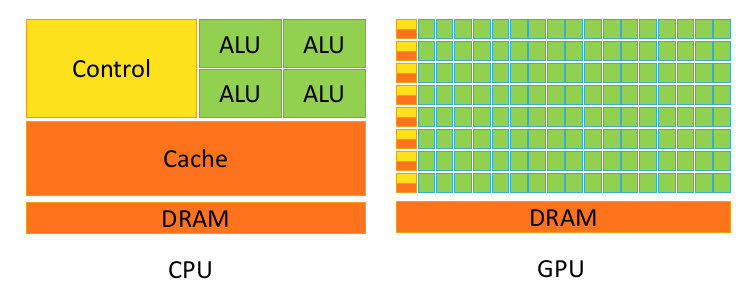
\includegraphics[width=1\linewidth]{CPUvsGPU.png}
    \caption{Differenza di architettura \cite{CUDAtutorial}}
\end{figure}

I \textbf{thread} della GPU sono molto più leggeri rispetto a quelli della CPU, il che rende più efficiente il loro passaggio da uno all'altro. Anche se le latenze possono essere più elevate, la capacità di commutare rapidamente i thread e di gestire più istruzioni in parallelo permette alla GPU di mantenere un \textbf{throughput elevato} durante l'elaborazione. Pertanto, i vantaggi di utilizzare le GPU per calcoli intensivi aumentano all'aumentare del numero di thread impiegati per un determinato compito.

\section{Il modello di esecuzione di CUDA}

Nel modello di esecuzione di CUDA esistono due tipi di funzioni principali:

\begin{itemize}
    \item \texttt{\_\_global\_\_}: Queste funzioni sono chiamate \textit{kernel functions} e possono essere invocate dalla \textit{host} (CPU) per essere eseguite sulla \textit{device} (GPU). Sono definite con il qualificatore \texttt{\_\_global\_\_} e devono essere invocate con una sintassi speciale, specificando il numero di thread e blocchi da lanciare. Una caratteristica particolare delle funzioni \texttt{\_\_global\_\_} è che il loro tipo di ritorno deve essere sempre \texttt{void}. Ecco un esempio di dichiarazione di una funzione \texttt{\_\_global\_\_}:

    \begin{lstlisting}
    __global__ void myKernel(int *data) {
        // Codice da eseguire sulla GPU
    }
    \end{lstlisting}

    \item \texttt{\_\_device\_\_}: Queste funzioni possono essere chiamate solo da altre funzioni eseguite sulla \textit{device} (ovvero dalla GPU stessa) e non possono essere invocate direttamente dalla \textit{host}. Le funzioni \texttt{\_\_device\_\_} sono eseguite sulla GPU e possono avere qualsiasi tipo di ritorno. Ecco un esempio di dichiarazione di una funzione \texttt{\_\_device\_\_}:

    \begin{lstlisting}
    __device__ int square(int x) {
        return x * x;
    }
    \end{lstlisting}
\end{itemize}

\chapter{Panoramica della localizzazione e mappatura simultanea }

\section{Python}

È un linguaggio di programmazione ad alto livello, interpretato e
orientato agli oggetti, che si è rapidamente affermato come uno degli
strumenti più versatili e popolari per lo sviluppo software, grazie alla
sintassi semplice e leggibile, che lo rende accessibile sia ai
programmatori principianti che agli esperti.\\
Creato da Guido van Rossum e rilasciato per la prima volta nel 1991,
Grazie alla sua vasta libreria standard e alla forte comunità di
supporto, Python è utilizzato in una vasta gamma di applicazioni, che
spaziano dl web development all'automazione di script, dalla data science all'intelligenza artificiale."

\section{MicroPython}

MicroPython d'altra parte, è una reimplementazione di
Python pensata specificamente per i microcontrollori e i dispositivi a
risorse limitate. MicroPython conserva la semplicità e la leggibilità di
Python, ma è ottimizzato per funzionare in ambienti dove memoria,
potenza di calcolo e risorse sono estremamente limitate. MicroPython
permette di scrivere codice Python standard, ma è dotato anche di moduli
e funzionalità specifiche per interagire direttamente con
l'hardware, come GPIO, PWM, I2C e SPI, che sono
comunemente utilizzati nei progetti di elettronica embedded.

La comparazione tra MicroPython e Python classico si focalizza
principalmente sulle prestazioni, sul consumo di risorse e sulle
applicazioni d'uso. Mentre Python viene eseguito su
computer con capacità hardware relativamente elevate, MicroPython è
progettato per essere eseguito su microcontrollori con pochi kilobyte di
memoria, come il chip ESP8266 o l'ESP32, che lo rende
ideale per applicazioni in Internet of Things (IoT) e automazione.
Pertanto, la differenza principale risiede
nell'ottimizzazione: MicroPython sacrifica alcune
funzionalità avanzate e performance rispetto a Python standard per
adattarsi alle limitazioni dell'hardware embedded.

In questa tesi, verranno analizzate le differenze di performance tra
MicroPython e Python in vari contesti, esplorando in che modo ciascuna
implementazione può essere più vantaggiosa a seconda delle esigenze
specifiche del progetto. Verranno esaminati casi di studio pratici per
illustrare l'uso di MicroPython in ambienti embedded e
saranno presentati test comparativi per valutare
l'efficienza delle due implementazioni in scenari
tipici.

\section{Differenze tra Python e MicroPython}

Python e MicroPython, sebbene condividano gran parte della sintassi e dei concetti fondamentali, presentano differenze significative a causa delle diverse finalità di utilizzo. MicroPython è stato progettato per microcontrollori e dispositivi con risorse limitate, mentre Python viene solitamente eseguito su computer o server con molta più potenza di calcolo e memoria.

\subsection{Dimensioni dell'interprete e Ottimizzazione per dispositivi embedded}

La caratteristica distintiva di MicroPython è la sua leggerezza. L'interprete di MicroPython è molto più piccolo di quello di Python, tipicamente occupando meno di 512 KB di memoria flash, a seconda della configurazione e delle librerie incluse. Python, al contrario, richiede molto più spazio a causa della sua vasta libreria standard e delle sue funzionalità avanzate.

MicroPython è progettato per essere eseguito in ambienti embedded, come microcontrollori e dispositivi a risorse limitate, dove memoria RAM e flash sono estremamente ridotte. Per fare questo, MicroPython esclude alcune caratteristiche di Python standard e include una gestione ottimizzata della memoria, con un garbage collector progettato per lavorare con quantità di RAM molto limitate.

\subsection{Libreria Standard}

Python è noto per la sua vasta libreria standard che copre una gamma estremamente ampia di funzionalità, dal networking all'elaborazione del testo, fino all'interfacciamento con database. MicroPython, invece, include solo un sottoinsieme della libreria standard di Python, limitato a ciò che è strettamente necessario per lavorare in ambienti embedded.

Le librerie disponibili in MicroPython sono adattate per essere utilizzate su microcontrollori e comprendono moduli specializzati per l'interazione diretta con l'hardware. Alcuni di questi moduli includono il supporto per GPIO, I2C, SPI e UART, funzioni essenziali per il controllo di dispositivi e sensori esterni, che non fanno parte del Python standard.

Successivamente si analizzeranno più in dettaglio le librerie disponibili nell'ambiente Micropython e eventuali alternative a popolari librerie Python.

\subsection{Gestione delle eccezioni e Debugging}

Python offre meccanismi avanzati per la gestione delle eccezioni e strumenti di debugging come pdb, che permettono di tracciare gli errori e risolvere i problemi nel codice in modo dettagliato. In MicroPython, la gestione delle eccezioni è semplificata per risparmiare risorse, e alcune delle funzionalità avanzate di debugging non sono disponibili, come ad esempio il supporto completo per il traceback approfondito.

Inoltre, per ridurre l'overhead, MicroPython può escludere le informazioni di debugging come i nomi dei file e i numeri di linea nel traceback, rendendo il debugging meno dettagliato rispetto a Python. Tuttavia, MicroPython fornisce strumenti di base per individuare errori, come i messaggi di errore semplificati e la stampa dello stato del programma.

\subsection{Gestione della memoria e Garbage Collector}

MicroPython utilizza un garbage collector più semplice rispetto a Python, ottimizzato per funzionare in dispositivi con memoria limitata. L'allocazione dinamica della memoria viene gestita in modo molto più conservativo rispetto a Python standard, e il garbage collector viene eseguito in modo esplicito o automatico quando necessario per liberare la memoria occupata da oggetti non più utilizzati.

\subsection{Reattività e Tempo Reale}

Un altro aspetto chiave di MicroPython è la sua capacità di operare in tempo reale su microcontrollori. Poiché MicroPython è eseguito direttamente sull'hardware senza un sistema operativo completo, è possibile scrivere codice che risponde in modo rapido e deterministico agli eventi hardware, come la gestione di interrupt o il controllo di motori e sensori. Python, essendo generalmente eseguito su sistemi operativi, non è ottimizzato per operare in ambienti real-time e dipende dal kernel del sistema operativo per la gestione delle operazioni hardware.

\chapter{Esperimenti e scopo della ricerca}

\section{Installazione di
MicroPython}\label{installazione-di-micropython}

Essendo un progetto open source è possibile scaricare il sorgente
direttamente da GitHub. In alternativa sono presenti anche pacchetti già
compilati per alcune distribuzioni Linux e per le schede già
supportate.\\
Debian SID: \cite{debian_sid} \\
AUR:\cite{aur_arch} \\
Nella documentazione di MicroPython \cite{micropython_getting_started} è presente la guida ufficiale per
l'installazione da sorgente, che può essere eseguita
seguento i seguenti passi:

\begin{enumerate}
\item
  clone del progetto
\begin{verbatim}
git clone https://github.com/micropython/micropython}
\end{verbatim}
\item
  compilazione del port per unix
\begin {verbatim} 
cd micropython/ports/unix
make submodules
make
\end{verbatim}
\end{enumerate}

\begin{enumerate}
\setcounter{enumi}{2}
\item
  alla fine della compilazione sarà presente
  l'eseguibile \texttt{micropython} nella directory
  \texttt{build-standard}
\end{enumerate}

\section{Package management}

Essendo non completamente compatibile con python i package compatibili
con MicroPython sono molto limitati rispetto a quelli offerti per
Python.\\
Per installare pacchetti per MicroPython non si utilizza pip, ma un
package manager apposito chiamato MIP \cite{MIP}
(Mip Installs Packages)\\
MIP permette alle board che possiedono una connessione internet di
installare pacchetti necessari.\\
A differenza di pip MIM non si appoggia al PyPI index ma utilizza di
default l'index micropython-lib \cite{micropython_lib}

\subsection{Pacchetti micropython-lib}\label{pacchetti-micropython-lib}

dalla pagina del progetto \cite{micropython_lib} si può vedere come i pacchetti disponibili siano divisi in
4 sezioni:

\begin{enumerate}
\item
  python-stdlib: implementazioni della standard library di Python \cite{python_standard_library}

  \begin{itemize}
    \item
    questi moduli hanno l'obiettivo di far girare codice
    Python su MicroPython

    \begin{itemize}
        \item
      viene comunque fatto notare che la la compatibilità non è
      perfetta, quindi ci saranno comunque delle limitazioni
    \end{itemize}
  \end{itemize}
\item
  python-ecosys: porting di librerie dell'ecosistema Python
  \begin{figure}
    \centering
    \includegraphics[width=1\linewidth]{libraries.png}
    \caption{python-ecosys}
\end{figure}
  \begin{itemize}
    \item
    sfortunatamente la collezione è estremamente ridotta con solo questi
    pacchetti presenti:
    
  \end{itemize}
\item
  Micropython: librerie specifiche di MicroPython, per controllo
  perifiche, sensori ecc...
\item
  unix-ffi: librerie utili per il porting di micropython su unix
\end{enumerate}

in conclusione l'index micropython-lib, eccetto per le
librerie standard, offre \textbf{poco supporto} per le librerie più
conosciute dell'ecosistema Python come Pandas, NumPy,
TensorFlow...\\
Le librerie sopracitate non offrono inoltre metodi alternativi per
l'installazione e l'utilizzo su
Micropython.

\section{Librerie alternative}

Come anticipato, risulta che non ci sia un modo diretto di utilizzare
le librerie dell'ecosistema di Python su Micropython, ma
devono solitamente essere \textbf{appositamente sviluppate} o è
necessario fare un porting.\\
I problemi principali dell'incompatibilità sono due:

\begin{enumerate}
\item
  le C extension

  \begin{itemize}
    \item
    la maggior parte delle librerie popolari di Python utilizzano
    estensioni di C per le performance, visto il cambio di piattaforma,
    queste non sono spesso portabili sui microcontrollori
  \end{itemize}
\item
  feature di Python\\
  - nonostante MicroPython (specialmente grazie
  all'index micropython-lib) offra la maggior parte
  delle feature di Python, la compatibilità non è completa\\
  Si decide quindi di analizzare l'ecosistema di
  MicroPython, per analizzare la situazione
\end{enumerate}

\subsection{Machine learning}\label{machine-learning}

Le librerie più comuni per il machine learning (numpy, scipy,
sickit-lean) non sono utilizzabili con MicroPython, ma sono disponibili
alternative:

\begin{itemize}
\item
  {ULAB}\cite{ulab}:
  offre un subset limitato di numpy e scipy

  \begin{itemize}
    \item
    l'obiettivo del progetto è
    l'implementazione di funzioni di queste librerie
    mentendo un'utilizzo della RAM limitato ma
    mantenendo alte performance
  \item
    il progetto non punta non punta a coprire tutte le funzionalità di
    numpy e scipy, ma solo di implementare quelle che ha senso
    utilizzare in un contesto embedded
  \end{itemize}
\item
  Emlearn \cite{emlearn}: permette di fare
  il training in Python con librerie Scikit-learn or Keras e genera un
  header C99 senza particolari dipendenze, utilizzabile su
  microcontroller

  \begin{itemize}
    \item
    questa libreria non è quindi una libreria di MicroPython, ma
    permette
  \end{itemize}
\item
  Tensorflow\cite{openmv_tensor}: esiste
  una libreria tensorflow che supporta solo le schede OpenMV Cam
\end{itemize}

\subsection{Web}\label{web}

Le librerie più frequentemente utilizzate per lo scraping (BeatifulSoup)
o per la creazione di web server (Django, Flask) non sono presenti.\\
È però presente la famosa libreria requests per fare semplici
interrogazioni HTTP. E la libreria socket permette la creazione di un
HTTP server.\\
È anche disponibili la libreria html che fornisce funzioni utili per la
gestione e manipolazione di HTML.

\subsection{Calcolo scientifico}\label{calcolo-scientifico}

Per il calcolo scientifico è disponibile la libreria standard math ed è
possibile utilizzare la libreria ULAB \cite{ulab}
sopracitata che offre parte delle funzionalità di numpy e scipy

\chapter{ULAB}\label{ulab}

A seguito della panoramica delle librerie fatta in precedenza si è
deciso di procedere con l'approfondimento della libreria
ULAB, in quanto risulta avere una buona compatibilità con Numpy e Scipy,
due librerie fondamentali per il calcolo scientifico.\\
A seguito di una introduzione ci si concentrerà sullo studio della
compatibilità con le librerie sopracitate e con il testing delle
performance.

\section{Introduzione}\label{introduzione-1}

\textbf{ULAB} (MicroLab) è una libreria progettata per
l'ecosistema MicroPython, concepita per fornire
funzionalità simili a quelle offerte dalla popolare libreria
\textbf{NumPy} di Python, ma ottimizzate per
l'esecuzione su microcontrollori e dispositivi a risorse
limitate. ULAB consente agli sviluppatori di eseguire operazioni
matematiche e scientifiche avanzate direttamente su microcontrollori,
senza dover ricorrere a un hardware più potente o a linguaggi di
programmazione più complessi.

In contesti embedded, dove memoria e potenza di calcolo sono limitate,
le librerie standard di Python, come NumPy, non possono essere
utilizzate a causa della loro complessità e dei requisiti di risorse.
ULAB è stata sviluppata per colmare questa lacuna, offrendo un subset di
funzionalità simili a NumPy, ma con un footprint di memoria molto
ridotto e prestazioni ottimizzate per microcontrollori come ESP32,
STM32, e altri.

ULAB supporta una vasta gamma di operazioni, tra cui manipolazioni di
array, operazioni aritmetiche, funzioni matematiche avanzate, e
trasformate di Fourier. Queste funzionalità permettono agli sviluppatori
di eseguire calcoli direttamente sui dati acquisiti dai sensori o altre
fonti in tempo reale, rendendo possibile l'analisi e
l'elaborazione dei dati in applicazioni di Internet of
Things (IoT), robotica, automazione e molto altro.

Un aspetto cruciale di ULAB è la sua efficienza. Essendo progettata
specificamente per MicroPython, la libreria è estremamente leggera e
ottimizzata per eseguire operazioni matematiche con un overhead minimo.
Questo rende ULAB uno strumento indispensabile per coloro che sviluppano
applicazioni embedded che richiedono capacità di calcolo più avanzate
rispetto a quelle offerte nativamente da MicroPython, ma che non possono
permettersi l'uso di hardware più costoso o ingombrante.

In questa tesi, si esplorerà l'utilizzo di ULAB in
diversi scenari pratici, confrontando le sue prestazioni e capacità con
quelle delle librerie simili disponibili in Python standard. Verranno
presentati esempi applicativi per dimostrare come ULAB può essere
utilizzata per ottimizzare processi computazionali in ambienti embedded,
mantenendo un equilibrio tra efficienza e semplicità di sviluppo.

\section{Installazione di ULAB}\label{installazione-di-ulab}

ULAB, a differenza delle classiche librerie Python, non risulta essere
un modulo separato, ma permette di generare un nuovo firmware
MicroPython con la libreria ULAB integrata. ULAB offre infatti uno
script di build che è possible lanciare per
l'installazione.\\
Si illustrano i punti per la compilazione del firmware Unix, come
descritto nel README del progetto \cite{ulab_compiling}

\begin{enumerate}
\item
  clone del progetto
\end{enumerate}

\begin{verbatim}
    git clone https://github.com/v923z/micropython-ulab.git ulab
\end{verbatim}

\begin{enumerate}
\setcounter{enumi}{1}
\item
  entrare nella cartella del progetto
\end{enumerate}
\begin{verbatim}
    cd ulab
\end{verbatim}

\begin{enumerate}
\setcounter{enumi}{2}
\item
  compilazione del firmware\\
  \texttt{bash\ ./build.sh\ 2\ }\strut \\
  - il parametro \texttt{2} indica la dimensionalità massima degli
  ndarray, successivamente verrà analizzata più in dettaglio questa
  proprietà\\
  - il valore può variare da 1 a 4, dove 2 è il default
\item
  verrà creata la directory
  \texttt{./micropython/ports/unix/build-\{n\}/} in cui si troverà
  l'eseguibile \texttt{micropython-\{n\}}, dove
  \texttt{\{n\}} è il valore del parametro specificato precedentemente
\item
  nel caso si fosse eseguito il comando al punto 3 come indicato, a fine
  della compilazione sarà possibile avviare il firmware eseguendo il
  seguente comando
\begin{verbatim}
    ./micropython/ports/unix/build-2/micropython-2
\end{verbatim}
\end{enumerate}

Il firmware generato sarà un'eseguibile stand-alone con
dipendenze molto ridotte. Per Debian Bookworm basterà assicurarsi di
aver installato il pacchetto \texttt{binutils}

\section{Configurabilità di ULAB}

ULAB permette di configurazione il firmware in modo da adattarlo alle
caratteristiche della propria scheda e alle esigenze del programma che
dovrà girarci.\\
Per la configurazione ULAB utilizza l'header
\texttt{ulab.h} accessibile nella directory \texttt{code} del progetto
di ULAB. Nell'hein cui sono presenti\\
I parametri sono specificati nel file \texttt{ulab.h} come define.

\subsection{Dimensioni matrici}\label{dimensioni-matrici}

\texttt{ULAB\_MAX\_DIMS} indica la dimensionalità massima delle matrici
supportate dal firmware.\\
Il valore può andare da 1 a 4, di default è specificato il valore 2.\\
Questo è il parametro che più impatta la dimensione e la funzionalità
del firmware. È quindi buona norma settare un valore che rispetti le
esigenze del programma utilizzato. Utilizzare un firmware con
dimensionalità troppo alta potrebbe portare ad un aumento considerevole
della dimensione come si vedrà in seguito.

Questo parametro può essere anche specificato al momento della
compilazione del firmware per unix, come parametro del comando
\texttt{build.sh}, esempio:

\begin{verbatim}
    ./build.sh [matrix.dims]
\end{verbatim}

\subsection{Altri parametri}\label{altri-parametri}

\begin{itemize}
\item
  \texttt{NDARRAY\_HAS\_BINARY\_OPS} abilita la presenza degli operatori
  binari per gli ndarray, a costo di un aumento della dimensione del
  firmware

  \begin{itemize}
    \item
    valore di default: 0
  \end{itemize}
\item
  \texttt{ULAB\_HAS\_FUNCTION\_ITERATOR} indica di scrivere le
  iterazioni sulle dimensioni degli array come funzioni, invece che con
  macro, risparmiando spazio al costo di performance

  \begin{itemize}
    \item
    valore di default: 0
  \end{itemize}
\item
  \texttt{NDARRAY\_IS\_ITERABLE} abilita la funzione di iterazione degli
  ndarry, risparmiando spazio

  \begin{itemize}
    \item
    valore di default: 1
  \end{itemize}
\item
  \texttt{NDARRAY\_IS\_SLICEABLE} abilita lo slicing degli ndarray

  \begin{itemize}
    \item
    valore di default: 1
  \end{itemize}
\item
  \texttt{NDARRAY\_BINARY\_USES\_FUN\_POINTER} abilita
  l'utilizzo di puntatori a funzione nelle iterazoni
\item
  \texttt{ULAB\_HAS\_DTYPE\_OBJECT} determina se il dtype è un oggetto o
  un carattere, la rappresentazione con l'oggetto è più
  compatibile con Numpy, ma occupa più spazio.
\end{itemize}

\chapter{Performance testing}

Si è quindi deciso di testare vari versione del firmware analizzando lo
spazio occupato e le performance e confrontarli con python

\section{Ambiente di testing}

I testing sono stati fatti su ambiente docker con distribuzione Debian
Bookworm.\\

\section{Firmware testati}

Intanto si definiscono i due firmware di reference per performance e
dimensione:

\begin{enumerate}
\item
  \texttt{python3}: CPython 3.11 desktop, versione installata su Debian
  Bookworm
\item
  \texttt{ulab-2}: MicroPython versione 3.4\\
  1. tutti i parametri sono stati lasciati al valore di default\\
  2. questo è il firmware di reference per MicroPython\\
  Successivamente si è deciso di cambiare la dimensionalità massima
  delle matrici cambiando la macro \texttt{ULAB\_MAX\_DIMS}, ma
  lasciando tutti gli altri parametri invariati, generando i seguenti
  firmware:
\item
  \texttt{ulab-3}: firmware ULAB, con dimensionalità massima 2
\item
  \texttt{ulab-4}: firmware ULAB, con dimensionalità massima 4\\
  Successivamente, tenendo come riferimento la dimensionalità massima 3,
  si è deciso di generare i seguenti firmware per valutare
  l'impatto dei parametri sopracitati nelle performance
  e nello spazio ottenuto. Questi sono i firmware risultanti:
\end{enumerate}

\begin{itemize}
\item
  \texttt{ulab-2\_has\_binary\_ops\_0}: la macro
  NDARRAY\_HAS\_BINARY\_OPS è settata a 0
\item
  \texttt{ulab-2\_has\_function\_iterator\_1}: la macro
  ULAB\_HAS\_FUNCTION\_ITERATOR è settata a 1
\item
  \texttt{2\_ndarray\_is\_iterable\_0}: la macro NDARRAY\_IS\_ITERABLE è
  settata a 0
\item
  \texttt{ulab-2\_ndarray\_is\_sliceable\_0}: la macro
  NDARRAY\_IS\_SLICEABLE è settata a 0
\item
  \texttt{ulab-2\_ndarray\_uses\_fun\_pointer\_1}: la macro
  \texttt{NDARRAY\_BINARY\_USES\_FUN\_POINTER} è settata a 1
\item
  \texttt{ulab-2\_ulab\_has\_dtype\_object\_1}: la macro
  \texttt{ULAB\_HAS\_DTYPE\_OBJECT} è settata a 1
\end{itemize}

\section{Analisi dimensione firmware}


Si presenta un grafico di comparazione delle dimensioni dei diversi firmware:
\begin{figure}
    \centering
    \includegraphics[width=1\linewidth]{size.png}
    \caption{Dimensioni firmware}
\end{figure}
Si presenta anche una versione tabellare dei dati graficati,
visualizzati in ordine decrescente di dimensione:

\begin{center}
\begin{tabular}{|c | c | c |}
\hline
firmware & size (Kb) & SLOC \\
\hline
python3 & 23616 & 6881 \\
ulab-4 & 6636 & 188787 \\
ulab-3 & 6504 & 180699 \\
ulab-2 & 6368 & 172502 \\
ulab-2\_has\_function\_iterator\_1 & 5640 & 178862 \\
ulab-2\_ulab\_has\_dtype\_object\_1 & 5552 & 173460 \\
ulab-2\_has\_binary\_ops\_0 & 5548 & 173212 \\
ulab-2\_ndarray\_is\_iterable\_0 & 5544 & 173158 \\
ulab-2\_ndarray\_is\_sliceable\_0 & 5520 & 172032 \\
ulab-2\_ndarray\_uses\_fun\_pointer\_1 & 5520 & 171419 \\
\hline
\end{tabular}
\end{center}

Dove con SLOC (Single Lines Of Code) si intendono le linee di codice Assembly del firmware.

Si può innanzitutto osservare che l'eseguibile Python
risulta di un ordine di grandezza più grande rispetto ai firmware
Micropython.\\
È chiaramente visibile come l'aumento della
dimensionalità delle aumenti lo spazio necesario, e come il cambiamento di
oguno dei valori di default delle macro porti ad una diminuzione della dimensione del firmware.

\subsection{Importanza delle SLOC}

È importante considerare la dimensione del firmware non solo perché un firmware più piccolo può essere caricato in una memoria limitata. Un firmware di dimensioni ridotte è anche più semplice da certificare, aspetto fondamentale in molte applicazioni critiche. La semplificazione della certificazione deriva dal fatto che un codice più piccolo è più facile da analizzare e verificare in tutte le sue parti.

In questo contesto, è stata prestata particolare attenzione anche al numero di istruzioni in assembly. In settori come la robotica biomedica, dove ogni componente del sistema deve essere estremamente affidabile, certificare l'intero firmware diventa essenziale. Avere un controllo preciso sul numero di istruzioni e sulla loro esecuzione aiuta a garantire che il sistema operi in modo sicuro e conforme alle normative.


\section{Descrizione test performance}\label{descrizione-test-performance}

I test eseguiti avevano l'obiettivo di utilizzare
diverse funzione di Numpy/ULAB.\\
I test sono stati eseguiti utilizzando un unico script Python
compatibile sia con CPython con librerie Numpy e Scipy, che con
MicroPython utilizzando con libreria ULAB.\\
Tutti i test sono ripetuti 100 volti per assicurarsi di eliminare
outliers\\
Lo script esegue 4 test che sono:

\begin{itemize}
\item
  matrix multiplication
\item
  interpolation
\item
  fft
\item
  linear system
\end{itemize}

\subsection{Matrix multiplication}\label{matrix-multiplication}

Si esegue una moltiplicazione tra due matrici 200 x 200, utilizzando la
funzione \texttt{np.dot()}

\subsection{Interpolation}\label{interpolation}

Interpolazione di due vettori di 100000 elementi, utilizzando la
funzione \texttt{np.interp()}

\subsection{FFT}\label{fft}

Calcolo della trasformata di Fourier di un vettore di 65536 elementi
utilizzando la funzione \texttt{np.fft.fft()}

\subsection{Linear system}\label{linear-system}

Risoluzione di un sistema lineare di equazioni composto da due matrici
di 800 elementi.\\
Questo test è l'unico dei 4 per cui è stato necessario
differenziare il codice per Numpy e ULAB, in quanto la funzione
\texttt{cho\_solve} di ULAB prende la matrice A, mentre per la stessa
funzione di Scipy è necessario prima fattorizzare A attraverso la
funzione \texttt{cho\_factor}

\section{Risultati test di performance}\label{risultati-test-di-performance}

Si mostrano i risultati dei test di performance per tutti i firmware: \\

\begin{figure}[h!]
    \centering
    \includegraphics[width=1\linewidth]{performance.png}
    \caption{Test performance}
\end{figure}

qui si mostra, in ordine di velocità i firmware più performanti:


\begin{center}
\begin{tabular}{|c | c | c | c | c |}
\hline
firmware & min & max & median & std \\
\hline
python3 & 2.88771 & 839.135751 & 7.363561 & 117.306519 \\
ulab-2\_ndarray\_uses\_fun\_pointer\_1 & 6.69400 & 62.516000 & 12.849500
& 16.539355 \\
ulab-2\_has\_binary\_ops\_0 & 7.16300 & 56.928000 & 13.210500 &
14.668942 \\
ulab-2\_ulab\_has\_dtype\_object\_1 & 7.07300 & 52.117000 & 13.451000 &
14.362896 \\
ulab-2\_ndarray\_is\_iterable\_0 & 7.01100 & 52.777000 & 13.816000 &
14.325753 \\
ulab-4 & 6.33800 & 46.979000 & 14.359500 & 14.066975 \\
\textbf{ulab-2} & \textbf{6.46000} & \textbf{55.938000} &
\textbf{14.440000} & \textbf{15.599915} \\
ulab-2\_ndarray\_is\_sliceable\_0 & 6.95900 & 51.058000 & 14.914000 &
14.494034 \\
ulab-3 & 5.96900 & 57.900000 & 15.252500 & 14.811854 \\
ulab-2\_has\_function\_iterator\_1 & 6.30600 & 54.867000 & 15.292000 &
14.323220 \\
\hline
\end{tabular}
\end{center}

Salta subito all'occhio CPython, con performance
considerevolmente maggiori rispetto agli altri firmware.\\
Successivamente si può osservare che nessun firmware customizzato ha
peggiorato considerevolmente le performance rispetto a ulab-2 (il
firmware di reference), alcuni hanno anche migliorato le performance.

\subsection{Analisi performance Python nel test "linear-system"}

Inaspettatamente la performance di CPython nel test "linear system" è
considerevolmente peggiore rispetto agli altri firmware, rendendolo
l'unico test in cui le performance di CPython sono
inferiori a quelle di Micropython.\\
Analizzando più approfonditamente la questione il problema sembra essere
abbastanza evidente:


\begin{center}
\begin{tabular}{|c | c | c | c | c | c |}
\hline
firmware & min & max & median & std \\
\hline
python3 & 7.139038 & 839.135751 & 10.702393 &212.959248 \\
ulab-2 & 6.460000 & 8.041000 & 6.588000 & 0.281956 \\
\hline
\end{tabular}
\end{center}

Guardando questi valori si vede che il tempo massimo di CPython è molto
alto essendo più di 100 volte maggiore al valore massimo di ulab-2, il
valore minimo invece è abbastanza in linea con quello di ulab-2 con una
differenza di meno di un millisecondo. Questo ovviamente porta ad
un'altra deviazione standard.

Facendo riferimento a quanto presentato prima questo test è
l'unico per cui il codice è diverso tra MicroPython e
CPython, a causa della differenza di implementazione dei due.

Isolando il test si può infatti osservare come la maggior parte del
tempo sia preso nella fattorizzazione di cholesky, mentre il tempo di
risoluzione è molto basso.\\
Qui si mostra un esempio dei tempi di esecuzione di entrambe le parti:

\begin{center}
\begin{tabular}{|c | c | c |}
\hline
 &fattorizzazione & risoluzione \\
\hline
tempo (ms) & 99.856444 & 2.309838 \\
\hline
\end{tabular}
\end{center}

I tempi però si abbassano considerevolmente nelle iterazioni
successive.\\
Come si può vedere da i tempi di esecuzione delle varie iterazioni si ha
una considerevole riduzione dei tempi di esecuzione a seguito della nona
iterazione, che viene mantenuta fino alla fine:

\begin{center}
\begin{tabular}{|c | c | c |}
\hline
iterazione & tempo (ms) \\
\hline
1 & 839.135751 \\
2 & 392.83769 \\
3 & 584.091132 \\
4 & 736.04277 \\
5 & 788.097906 \\
6 & 692.523665 \\
7 & 583.249705 \\
8 & 555.962178 \\
9 & 440.824691 \\
10 & 10.586065 \\
11 & 9.417711 \\
12 & 7.88812 \\
... & ... \\
\hline
99 & 34.799827 \\
\hline
\end{tabular}
\end{center}

Si sospetta che questo fenomeno sia dovuto da un caching del risultato

\subsubsection{Differenze di implementazione}

Come anticipato il test "linear system" mostra la non completa compatibilità tra la libreria ULAB e la libreria Scipy.
Analizzando il codice del test si possono notare le differnze:

\begin{verbatim}
if using_ulab:
    res = scipy.linalg.cho_solve(a, b)
else:  
    factor = scipy.linalg.cho_factor(a)
    res = scipy.linalg.cho_solve(factor, b)
\end{verbatim}

Per l'esecuzione dello stesso script su entrambi i tipi di firmware è stato necessario differenziare la chiamata della funzione 
\texttt{cho\_solve}. Facendo riferimento alla documentazione di ULAB sulla funzione \texttt{cho\_solve} \cite{ulab_cholesky} si 
può leggere questa frase: \textit{"As opposed to scipy, the function simply takes the Cholesky-factorised matrix"} esplicitando appunto che la funzione non è direttamente compatibile con la corrispondente funzione della libreria Scipy.\\

Analizzando più in dettaglio i tempi di esecuzione, si che la maggior parte del tempo di esecuzione delle prime iterazioni è impiegato nella fattorizzazione della matrice, ovvero il passaggio non necessario per MicroPython.

Questo è un buon esempio dell'accortezza che è necessario utilizzare per eseguire il porting di uno script da Python a MicroPython.


\subsection{Nota sui numeri complessi}

Dai risultati del test FFT si è osservato che i valori restituiti da MicroPython non risultano diversi in struttura rispetto ai valori di riferimento restituiti da Python.
In particolare si osserva che Python restituisce un array unico con il risultato, mentre Micropython restituisce un array contente due array differenti.\\
La motivazione è che ULAB di base non supporta i numeri complessi, ma invece ritorna il risultato creando un array per la parte reale ed un array per la parte complessa.\\
Seguendo le indicazioni presentate nella documentazione della funzione fft, si vede che è però possibile attivare questa funzionalità a costo dell'utilizzo del 50\% in più di RAM.

Per attivare la gestione dei numeri complessi è sufficinete assicurarsi che la macro \texttt{ULAB\_SUPPORTS\_COMPLEX} sia settata a 1 e assicurarsi di settare ad 1 anche la macro \texttt{ULAB\_FFT\_IS\_NUMPY\_COMPATIBLE}

\subsection{Errori di approssimazione}

Confrontando i valori ritornati dai test fatti si nota come in due test i valori siano considerevolmente differenti rispetto ai valori di riferimento generati da Python. Si parte ad analizzare i valori risultanti dal test linear system, qui si possono vedere i primi 3 elementi di ciascun firmware:

\begin{verbatim}
Python: [0.0, 0.006257822277847307,
            0.008343763037129748]
ULAB 2: [0.0, 0.003128911138923654,
            0.002781254345709915]
\end{verbatim}

È subito evidente una considerevole differenza, al punto che persino la cifra significativa risulta differente.
Si nota un comportamento simile anche per il test fft:

\begin{verbatim}
Python: [(-1.4026391268080751e-14+0j),
            (1.570784341276565-32767.74994789285j),
            (-6.391749161391903e-05+0.6666836188068311j)]
ULAB 2: [(5.122156919054285e-08+0j),
            (1.570784369533921-32767.7499478676j),
            (-6.38901903868286e-05+0.666683635324262j)]
\end{verbatim}

Qui l'impatto sembra più ridotto, visto che per alcuni valori la corrispondenza è esatta, ma l'alcuni errori sono comunque presenti. \\
Per gli altri test invece non si osservano errori di approssimazione. Investigando meglio sulla problematica si ipotizza che il problema sia dovuto ad alcuni errori di approssimazione su MicroPython, che, anche se inizialmente molto piccoli, in base al tipo di operazione possono diventare sostanziali.

L'ipotesi si è verificata con la semplice radice di 2. Questo è il risultato di Pyhton:

\begin{verbatim}
1.41421356237309514547
\end{verbatim}

mentre questo è il risultato di Micropython:

\begin{verbatim}
1.41421356237309510107
\end{verbatim}

Dalla diciassettesima cifra decimale si nota infatti che i due valori divergono, introducendo quindi un errore nei calcoli. 
Si ipotizza che il motivo di questa differenza sia dato dal fatto che MicroPython, essendo più ottimizzato per lo spazio, sia capace di meno precisione rispetto a Python.

\chapter{Conclusioni}

In questa tesi, si è esplorato e confrontato l'uso di Python e MicroPython, con particolare attenzione alle applicazioni scientifiche e ai dispositivi a risorse limitate. Si è evidenziato come, sebbene Python sia un linguaggio versatile e potente, esso non risulti ottimizzato per ambienti con risorse ridotte, mentre MicroPython rappresenta una soluzione più efficiente e mirata in tali contesti.

Le principali differenze riscontrate riguardano le dimensioni dell'interprete, la gestione della memoria e la disponibilità delle librerie. MicroPython, grazie alla sua leggerezza e alla capacità di essere adattato all'hardware su cui viene eseguito, riesce a fornire molte delle funzionalità di Python, sacrificando alcune caratteristiche avanzate per garantire un uso ottimale delle risorse.

L'analisi comparativa delle prestazioni ha mostrato che MicroPython, in combinazione con librerie come ULAB, può essere una valida alternativa per operazioni scientifiche di base su sistemi embedded. I test eseguiti hanno dimostrato che, sebbene Python mantenga prestazioni superiori su piattaforme con risorse adeguate, MicroPython è in grado di competere efficacemente in ambienti a risorse limitate, specialmente quando si applicano ottimizzazioni specifiche.

Tuttavia, come emerso dai test relativi ai sistemi lineari e alle operazioni FFT, MicroPython presenta limitazioni in termini di precisione numerica rispetto a Python. Questo aspetto è rilevante nelle applicazioni in cui l'accuratezza dei calcoli è essenziale, come nella robotica o nel controllo industriale. Il compromesso tra precisione e prestazioni diventa, quindi, un fattore cruciale nella scelta della piattaforma di sviluppo per applicazioni embedded.

Un altro aspetto emerso riguarda la possibilità di personalizzazione del firmware. La configurabilità del firmware ULAB consente di adattarlo alle esigenze specifiche del dispositivo, offrendo flessibilità, ma richiede una comprensione approfondita delle opzioni di configurazione e delle esigenze del progetto. Come mostrato dai test, le variazioni nei parametri di compilazione possono influenzare significativamente sia le prestazioni sia le dimensioni del firmware, permettendo di bilanciare efficienza e capacità computazionale.

In conclusione, MicroPython offre un'ottima alternativa per coloro che necessitano di soluzioni Python-like in ambienti embedded con risorse limitate. Nonostante le limitazioni rispetto a Python standard, MicroPython, in combinazione con strumenti come ULAB, fornisce una base solida per lo sviluppo di applicazioni scientifiche e tecniche su microcontrollori. È però essenziale valutare attentamente le esigenze del progetto, considerando i compromessi in termini di precisione e prestazioni, al fine di scegliere la piattaforma più adatta. Questo secondo \cite{CUDAtutorial}


\bibliographystyle{apalike}
\bibliography{bibliografia}  % type -> @online,@misc,@unpublished,@thesis,@article,@book,...


\end{document}


